In this chapter, the rocket flight is modelled, and using this model a control loop consisting of a state estimation algorithm and a state feedback controller is designed.
The state estimation is realized with an EKF, and a gain scheduled LQR is used as feedback control.

\section{Modelling}
In this section the ``rocket-flight'' system will be modelled.
``Modelling'' means finding the underlying equations which describe the behaviour of the rocket in flight, its sensors and actuators, the environment, etc., and making assumptions and simplifications to ease the design of the control loop.
As the famous (and often repeated by my professors) quote goes
\begin{quote}
``All models are wrong, but some are useful'' - George Box
\end{quote}

Dynamical models of the rocket flight are needed for both the controller synthesis and the estimator algorithm.  
The rocket model is made up of a system of algebraic and differential equations \cite{zipfel2007, lewis2008, stevens2015}, represented in \textit{state-space} as \cite{lewis2008, stevens2015}
\begin{align}
    \dot x &= f(t, x, u) \label{eq:model-equation-f}  \\  
    y &= h(t, x, u) \label{eq:model-equation-h}
\end{align}  
with the state $x$, measurement output $y$, and control input $u$.
The state (or dynamics) equation $f$ and the output equation $h$ can be nonlinear functions, and may also depend on the time $t$\footnote{The equations will turn out to not depend explicitly on time, i.e. the differential equations \ref{eq:model-equation-f} may be treated as autonomous.}.
The equations are vector-valued, and the variables $x,u,y$ are vectors.

\textit{Linear time-invariant} (LTI) state-space models can be derived by linearizing the equations $f$ and $h$ around some point $(t_0, x_0, u_0)$, which results in the equations
\begin{align}
    \dot x = A (x-x_0) + B (u-u_0) \label{eq:model-linear-state} \\
    y = C (x-x_0) + D (u-u_0) \label{eq:model-linear-meas}
\end{align}
where the matrices $A,C$ are the Jacobians of $f,h$ with respect to the state $x$, and similar $C,D$ are Jacobians with respect to the input $u$.

The state $x$ is a collection of variables which describe the dynamics of the system in a collection of first order differential equations.\footnote{For example: a mass-spring-damper system has two state variables, position and velocity. These describe the energy stores of the system, potential of the deformed spring and kinetic of the moving mass.}
These states do not have to have a physical meaning \footnote{One could describe a system with its input-output relationship, without assigning a meaning to the variables of the differential equations.}, but will in this case as they describe the system well.
For aerospace vehicles, often chosen states are the attitude (Euler angles or quaternion), attitude rates, velocity, and position. 
The input signal $u$ describes how external sources influence the dynamics (and the measurement). 
This describes behaviour which is not captured by the state alone, for example actuators acting on the system.
The output signal $y$ describes how a certain state influences the environment.
This mostly encompasses measurements taken from the system by sensors.


\subsection{Kinematics and Quaternions}
\subsubsection{Coordinate frames}

The inertial frame $\mathrm{f}^G$ is assumed to be the earth-flat geographic frame, with an up-crossrange-downrange orientation (this is more useful than up-north-west).
The origin is located below the launch rail, with zero altitude at sea level.

The body-fixed frame $\mathrm{f}^B$ is oriented along the main inertia axes of the rocket body, namely forward-starboard-rail ($x^+$ is forward, and $z^+$ points toward the launch rail, downrange at launch), as shown in Figure \ref{fig:model-frame-rocket}.
The origin of the body-fixed frame is (as typical) located at the body center of gravity.

The sensor frames $\mathrm{f}^{S}$ are aboard the rocket, but rotated and translated against the body frame.

\begin{figure}[ht]
    \centering
    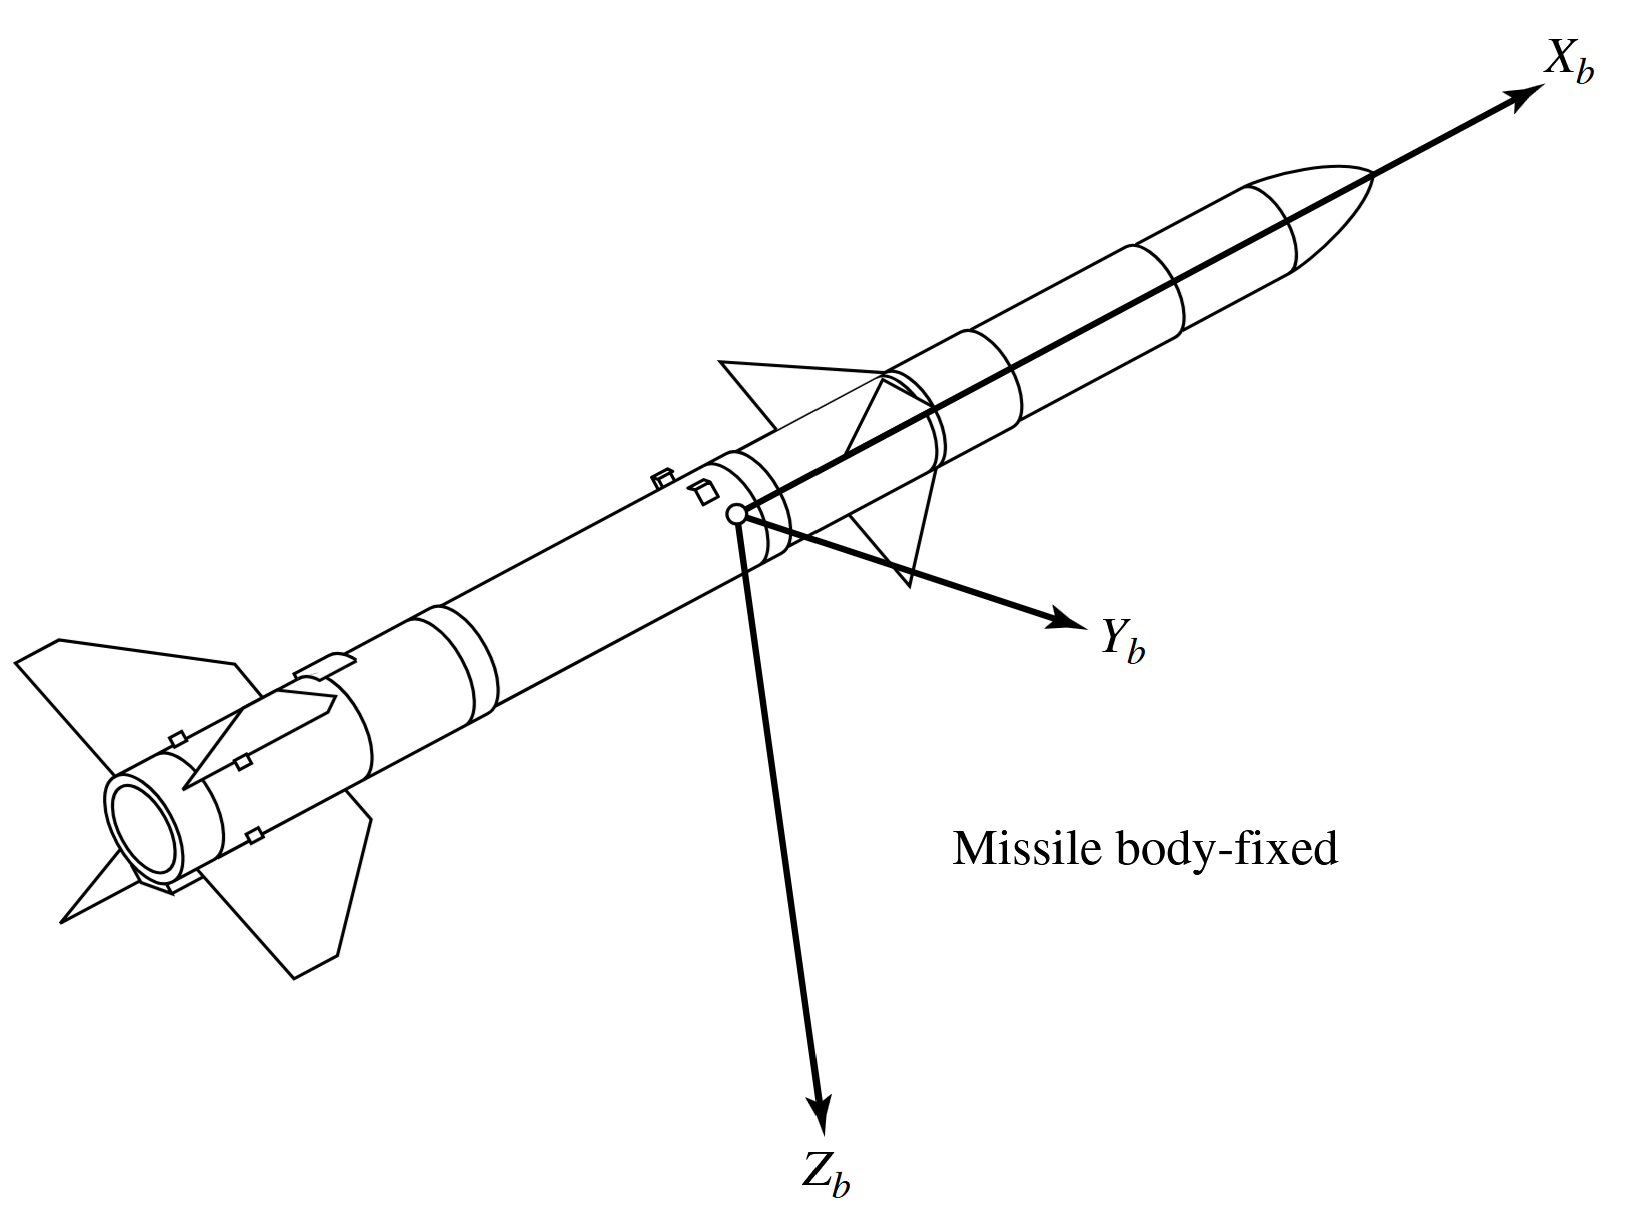
\includegraphics[width=0.45\linewidth]{images-design/model-coordinates-rocket.png}
    \caption[Diagram of the body-fixed frame $\mathrm{f}^B$]{Diagram of the body-fixed frame $\mathrm{f}^B$, taken from \cite{siouris2004}. (Here a different convention is used to denote the axes, $X_b$ rather than $x^B$). }
    \label{fig:model-frame-rocket}
\end{figure}

The rotational transformation of a vector $r$ between the frames is given by
\begin{align}
    r^G &= S r^B & r^B &= S^T r^G \\
    r^B &= S_i r^{S} & r^{S} &= S_i^T r^B 
\end{align}
with the rotation matrix $S$ (see Equation \ref{eq:rotationmatrix}), and the rotation matrix $S_i$ for the $i$-th sensor frame.
The frames $\mathrm{f}^G$ and $\mathrm{f}^B$ are shown in Figure \ref{fig:model-frames} with their rotation against each other.
To simplify the following notations, the velocities, the angular rates, and the external forces and torques are given in the body-fixed frame, and the index $^B$ is omitted.  
\begin{figure}[ht]
    \centering
    \resizebox{0.36\textwidth}{!}{
    \begin{tikzpicture}[scale=0.8, every node/.style={scale=0.2}, auto, node distance=1.5cm,>=latex']
        \tikzstyle{every node}=[font=\LARGE]

		%origin
		\coordinate(o) at (0,0) {};

		%earth coordinates
 		\node (X) at (0,12) {$x^G$};
        \draw [ ->] (o) -- (X);
        \node (Y) at (-6,-3) {$y^G$};
        \draw [ ->] (o) -- (Y);
		\node (Z) at (8,-4) {$z^G$};
        \draw [ ->] (o) -- (Z);
        		
		%box
		\coordinate(xx) at (0,10) {};
		\coordinate(yy) at (-4,-2) {};        
		\coordinate(zz) at (6,-3) {};
		\coordinate(yz) at (2,-5) {};
		\coordinate(xy) at (-4,8) {};
		\coordinate(xz) at (6,7) {};
		\coordinate(xyz) at (2,5) {};
		\draw [dotted] (yy) -- (yz);
		\draw [dotted] (zz) -- (yz);
		\draw [dotted] (xx) -- (xy);
		\draw [dotted] (yy) -- (xy);
		\draw [dotted] (xx) -- (xz);
		\draw [dotted] (zz) -- (xz);
		\draw [dotted] (xy) -- (xyz);
		\draw [dotted] (xz) -- (xyz);
		\draw [dotted] (yz) -- (xyz);
        		
		%body coordinates		
		\node (x) at (2.2,5.5) {$x^B$};
		\draw [very thick, ->] (o) -- (x);
		\node (y) at (-0.6,-6) {$y^B$};
        \draw [very thick, ->] (o) -- (y);
        \node (z) at (5,-1) {$z^B$};
        \draw [very thick, ->] (o) -- (z);
		\draw [dashed, ->] (o) -- (xy);
		\draw [dashed, ->] (o) -- (xz);
		%\draw [dashed, ->] (o) -- (yz);
      
 		%angles
 		 \draw [very thick, ->] (0,8) arc (90:50:8);  
 		 \node (theta) at (3.1,8.2) {$\theta$}; 
 		 \draw [very thick, ->] (0,7) arc (90:116:7); 
 		 \node (psi) at (-1.7,7.5) {$\psi$}; 
		   \draw [very thick, ->] (-2,-1) arc (230:268:3); 
 		 \node (phi) at (-1.8,-2.2) {$\phi$}; 

 		 \draw [very thick, ->] (2,3.75) arc (20:300:0.6); 
 		 \node (phi) at (0.6,4.5) {$\omega_x$}; 
		   \draw [very thick, <-] (0.2,-3.8) arc (0:300:0.6); 
 		 \node (phi) at (-1.7,-4.2) {$\omega_y$}; 
		   \draw [very thick, <-] (3.6,-0.6) arc (0:300:0.6); 
 		 \node (phi) at (4,0.2) {$\omega_z$}; 

\end{tikzpicture}}
    \caption[Diagram of attitude frames]{Diagram of the attitude coordinate frames with Euler angles and body rates.}
    \label{fig:model-frames}
\end{figure}

% \begin{figure}[ht]
%     \centering
%     \resizebox{0.36\textwidth}{!}{
%     \tdplotsetmaincoords{70}{120} % Set viewing angles
\begin{tikzpicture}[tdplot_main_coords, scale=4]

% Define the axes
\draw[->] (0,0,0) -- (1.5,0,0) node[anchor=north east] {$y^G$};
\draw[->] (0,0,0) -- (0,1.5,0) node[anchor=north west] {$z^G$};
\draw[->] (0,0,0) -- (0,0,1.5) node[anchor=south] {$x^G$};

% Define rotated body-frame axes
\tdplotsetrotatedcoords{50}{40}{-10} % Rotation angles: φ (roll), ψ (yaw), θ (pitch), 
% axis lengths: 
\pgfmathsetmacro{\ax}{1.5}
\pgfmathsetmacro{\ay}{1}
\pgfmathsetmacro{\az}{1}

\draw[->,tdplot_rotated_coords] (0,0,0) -- (\ay,0,0) node[anchor=west] {$y^B$};
\draw[->,tdplot_rotated_coords] (0,0,0) -- (0,\az,0) node[anchor=west] {$z^B$};
\draw[->,tdplot_rotated_coords] (0,0,0) -- (0,0,\ax) node[anchor=south] {$x^B$};

% Mark center of gravity
\filldraw[black] (0,0,0) circle (0.5pt) node[anchor=north east] {};

\tdplotsetrotatedcoords{50}{40}{-10}

% projected rotations
% yaw pitch
\tdplottransformrotmain{0}{0}{\ax}
\draw[tdplot_main_coords,->,red!50] (0,0,0)
-- (\tdplotresx,0,\tdplotresz);

% yaw roll
\tdplottransformrotmain{\ay}{0}{0}
\draw[tdplot_main_coords,->,green!50] (0,0,0)
-- (\tdplotresx,0,\tdplotresz);

% pitch roll
\tdplottransformrotmain{0}{\az}{0}
\draw[tdplot_main_coords,->,blue!50] (0,0,0)
-- (0,\tdplotresy,\tdplotresz);

% Draw the angles
% yaw (ψ)
\tdplotsetrotatedcoords{-90}{-90}{0}
\tdplotdrawarc[->,tdplot_rotated_coords,red!50]{(0,0,0)}{0.6}{0}{28}{anchor=north}{$\psi$}
\tdplotdrawarc[->,tdplot_rotated_coords,green!50]{(0,0,0)}{0.6}{90}{136}{anchor=north}{$\psi$}

% pitch (θ)
\tdplotsetrotatedcoords{180}{90}{90}
\tdplotdrawarc[->,tdplot_rotated_coords,red!50]{(0,0,0)}{0.7}{90}{123}{anchor=south west}{$\theta$}
\tdplotdrawarc[->,tdplot_rotated_coords,blue!50]{(0,0,0)}{0.7}{180}{188.5}{anchor=south west}{$\theta$}

% roll (φ)
\tdplotsetrotatedcoords{0}{0}{0}
\tdplotdrawarc[->,tdplot_rotated_coords,blue!50]{(0,0,0)}{0.8}{90}{140}{anchor=south}{$\phi$}
\tdplotdrawarc[->,tdplot_rotated_coords,green!50]{(0,0,0)}{0.8}{0}{50}{anchor=south}{$\phi$}


\end{tikzpicture}}
%     \caption[Diagram of attitude frames 2]{Diagram of the attitude coordinate frames with Euler angles.}
%     \label{fig:model-frames2}
% \end{figure}

\subsubsection{Attitude with Quaternions}
In aeronautics Euler angles are often used for control design.
However, the kinematics of the Euler angles show singularities at certain orientations, and the notation with large rotation matrices from sines and cosines is cumbersome.
For this reason the attitude of the rocket will be described by quaternions, as
\begin{quote}
``these differential equations are a joy to implement, because they are linear, have no singularities, and number only four'' - Peter Zipfel \cite{zipfel2007}
\end{quote}

The Quaternion is defined as  
\begin{equation}
    q = \begin{bmatrix}
        q_w & q_x & q_y & q_z 
    \end{bmatrix}^T = 
    \begin{bmatrix}
        q_w \\ q_v
    \end{bmatrix}
\end{equation}
which consists of four variables, often named as the real part $q_w$, and the vector part $q_v$.\footnote{Formally, the quaternion is a four-dimensional complex number, instead of $a+\mathrm{i}b$ it is $q_w + \mathrm{i} q_x + \mathrm{j} q_y + \mathrm{k} q_z$, where all variable are orthogonal and $\mathrm{i}^2 = \mathrm{j}^2 = \mathrm{k}^2 = \mathrm{ijk} = -1$. This will not really be relevant for implementing the mechanics, but explains some weirdness of the calculations.}
The attitude quaternion is normed to $|q| = q^T q =  1$ to describe rotations.
This unit constraint has to be enforced in the filter process, e.g. by norming $q$ after integration \cite{sola2017} as $q = q / \mathrm{norm}(q)$, or by Baumgarte stabilization (implemented is the former).

Euler's rotation theorem states that every rotation sequence (or attitude difference) in 3D space can be expressed as a single rotation with angle $\varphi$ around a single axis $n$ (unit vector) \cite{zipfel2007}.
The quaternion can be understood as that rotation, with
\begin{align}
    q_w &= \cos(\frac{\varphi}{2}) 
    &
    q_v &= n \sin(\frac{\varphi}{2})
    \label{eq:rotation-theorem}
\end{align}

The inverse of a unit quaternion is simply the conjugate \cite{stevens2015, sola2017}, so 
\begin{align}
    q^{-1} = \begin{bmatrix}
        q_w \\ q_v
    \end{bmatrix}^{-1} = \begin{bmatrix}
        q_w \\ -q_v
    \end{bmatrix}
\end{align}

To rotate one attitude to another attitude, the attitude quaternions are multiplied using the Hamiltonian product $*$ .
This can also be applied to rotate vectors, but the rotation matrix $S$ (Equation \ref{eq:rotationmatrix}) is computationally more efficient.
Two quaternions $q, r$ are multiplied to quaternion $p$ as \cite{stevens2015}
\begin{align}
    p &= q * r = \tilde Q \cdot r &
    \tilde Q &= \begin{bmatrix}
        q_w & -q_x & -q_y & -q_z \\
        q_x & q_w & -q_z & q_y \\
        q_y & q_z & q_w & -q_x \\
        q_z & -q_y & q_x & q_w
    \end{bmatrix} 
    \label{eq:quaternion-mult}
\end{align}
with the matrix $\tilde Q$ stemming from the Hamiltonian product \cite{stevens2015}.
To note: this multiplication is not commutative ($q*r \neq r*q$).

The time derivative of the quaternion attitude, with angular rates $\omega$ described in the body-fixed frame, has multiple equal expressions \cite{zipfel2007, sola2017, stevens2015}
\begin{align}
    \dot q \;
    &= \; \frac{1}{2} q * \begin{bmatrix}
        0 \\ \omega
    \end{bmatrix} \;
    = \; \frac{1}{2} \tilde Q \cdot \begin{bmatrix}
        0 \\ \omega
    \end{bmatrix} \;
    = \; \frac{1}{2} \tilde \Omega \cdot q \;
    & 
    \tilde \Omega &= \begin{bmatrix}
        0 & -\omega_x & -\omega_y & -\omega_z \\
        \omega_x & 0 & \omega_z & -\omega_y \\
        \omega_y & -\omega_z & 0 & \omega_x \\
        \omega_z & \omega_y & -\omega_x & 0
    \end{bmatrix}    
    \label{eq:quaternion-deriv}
\end{align}

For integration to a discrete time update, multiple approaches can be used. 
The simplest method to implement is explicit Euler with posteriori norming, which assumes small time steps such that the quaternion norm does not deviate far from 1.
The most accurate discrete time form is probably geometric integration, which preserves the unit constraint for any time step size. It assumes constant angular velocity over the time step to calculate an incremental attitude change $dq_k$ \cite{sola2017} 
% Time integration leads to the discrete dynamics of a quaternion attitude, described by the rotation with an incremental attitude difference \cite{sola2017, stevens2015} 
\begin{align}
    q(t + dt) &= q(t) * dq(t,dt) 
    &\implies
    q_{k+1} &= q_k * dq_k \\
%    \label{eq:quaternion-update}
    dq_k &= \begin{bmatrix} \cos(\frac{d\varphi}{2}) \\ dn \sin(\frac{d\varphi}{2})
    \end{bmatrix}
    & d\varphi &= \lVert \omega(t) \rVert dt 
    & dn &= \frac{\omega(t)}{\lVert \omega(t) \rVert}
    \label{eq:quaternion-increment}
\end{align}
here $q_{k+1}$ is the approximate (first order truncated Taylor series) closed-form solution of the differential equation \ref{eq:quaternion-deriv}.
% Its explicit, first order, and maintains the unit constraint, thus this form will be used for time integration of the quaternion, rather than explicit Euler for the other derivatives (see Section \ref{sec:numerical-integration}).





% \begin{equation}
%     \begin{bmatrix}
%        \dot q_w \\ \dot q_v
%     \end{bmatrix} 
%     = \frac{1}{2}
%     \begin{bmatrix}
%         0 & -\omega^T  \\
%         \omega & - \tilde \omega
%     \end{bmatrix} \cdot 
%     \begin{bmatrix}
%         q_w \\ q_v
%     \end{bmatrix}
%     = \frac{1}{2}
%     \begin{bmatrix}
%         q_w & q_v^T  \\
%         -q_v & q_w \bm I + \tilde q_v
%     \end{bmatrix} \cdot 
%     \begin{bmatrix}
%         0 \\ \omega
%     \end{bmatrix}
%     \label{eq:quaternion-deriv}
% \end{equation}
% \begin{align}
%     \tilde \omega &= \begin{bmatrix}
%         0 & -\omega_z & \omega_y \\
%         \omega_z & 0 & - \omega_x \\
%         -\omega_y & \omega_x & 0
%     \end{bmatrix}    
%     &
%     \tilde q_v &= \begin{bmatrix}
%         0 & -q_z & q_y \\
%         q_z & 0 & -q_x \\
%         -q_y & q_x & 0
%     \end{bmatrix}  
% \end{align}

The rotation matrix is used to transform a vector from one attitude to another, i.e. for the transformation from the body-fixed frame to the inertial frame.
It can be computed directly from the quaternion \cite{zipfel2007, stevens2015}. 
The rotation matrix $S = S_{G \to B}$ (or often $S = S^B_G$) transforms a vector from the ground frame $G$ to the body-fixed frame $B$, and is computed as \cite{stevens2015}
\begin{align}
    S &= \begin{bmatrix}
         q_w^2 + q_x^2 - q_y^2 - q_z^2 & 2 q_w q_z + 2 q_x q_y & 2 q_x q_z - 2 q_w q_y \\
    2 q_x q_y - 2 q_w q_z & q_w^2 - q_x^2 + q_y^2 - q_z^2 & 2 q_w q_x + 2 q_y q_z \\
    2 q_w q_y + 2 q_x q_z & 2 q_y q_z - 2 q_w q_x & q_w^2 - q_x^2 - q_y^2 + q_z^2
    \end{bmatrix} \label{eq:rotationmatrix} \\
    &= 2 q_v q_v^T + (q_w^2-q_v^T q_v) I_3 - 2 q_w \tilde q_v \nonumber
\end{align}
The inverse transformation, i.e. from a vector in $B$ to a vector in $G$, is performed by inverting the transformation matrix. 
Luckily, the rotation matrix is always orthogonal, so $S^{-1} = S^T$, and thus $S^G_B = S^T$. 
Additionally, the inverse rotation matrix is the rotation matrix of the inverse quaternion, so $S^T(q) = S(q^{-1})$.
The rotation $R(q,v) = S(q) \, v$ is equivalent to the operation \cite{stevens2015}
\begin{align}
    \begin{bmatrix}
        0 \\ R(q,v)
    \end{bmatrix} &= q^{-1} * \begin{bmatrix}
        0 \\ v
    \end{bmatrix} *q
\end{align}

The Euler angles \textit{yaw} $\psi$, \textit{pitch} $\theta$, and \textit{roll} $\phi$ can be recovered from the rotation matrix elements (or directly from the quaternions). 
For the rotation sequence yaw $\to$ pitch $\to$ roll (order $z\to y \to x$, rotation around the respective new body axes) the Euler angles are  \cite{stevens2015}
\begin{align}
    \psi &= \mathrm{atan2}(S_{12}, S_{11}) &
    \theta &= \mathrm{arcsin}(-S_{13}) &
    \phi &= \mathrm{atan2}(S_{23}, S_{33}) 
    \label{eq:quaternion2euler}
\end{align}

For initialization, the quaternion is set according to Equation \ref{eq:rotation-theorem}, where $\varphi$ is the launch angle, and $n$ indicates the launch orientation (pitch or yaw) \footnote{Initialization with Euler angles is also possible, see \cite{stevens2015}, \cite[p. 126]{zipfel2007}}.
A typical initialization could be $\varphi = $ launch angle, and $n = [\begin{smallmatrix} 0 & 1 & 0 \end{smallmatrix}]^T$, i.e. the rocket is pitched downrange, and both yaw and roll are defined zero.

\subsubsection{Relative motion}
Using Newton's second law, the acceleration in the body-fixed frame is \cite{zipfel2007, stevens2015}
\begin{align}
    \dot v = \mathcal{F}/m - \omega \times v + S g^G
    \label{eq:model-vel-deriv}
\end{align}
which accounts for the derivation in the rotating body-fixed frame with the transport term $- \, \omega \times v$, and the vector of external forces $\mathcal{F}$ ( in the body-fixed frame).
The gravity vector $g^G = \begin{bmatrix} -g_0 & 0 & 0 \end{bmatrix}^T$ is transformed to the body-fixed frame to account for the gravitational acceleration (magnitude $g_0 \approx 9.81 \frac{\mathrm{m}}{\mathrm{s}^2}$).
To note: gravity is thus not a part of the external forces $\mathcal{F}$.

The velocity in the inertial (geographic) frame is \cite{zipfel2007}
\begin{equation}
    \dot r^G = S^T v
    \label{eq:model-pos-deriv}
\end{equation}

With Euler's law, the angular acceleration is \cite{zipfel2007, schiehlen2017}
\begin{align}
   \dot \omega = J^{-1} (\mathcal{T} - \omega \times J \omega)
   \label{eq:model-rate-deriv}
\end{align}
which includes the external torques (or moments) $\mathcal{T}$ (described in the body-fixed frame) and the gyroscopic moment.
The inertia tensor $J$ is determined from CAD or experimentally. If the coupling inertia moments are very small, they may be neglected to fill the tensor diagonally as $J = \text{diag}\begin{bmatrix} J_x & J_y & J_z \end{bmatrix}$, where in a rocket cruciform typically $ J_x < J_y = J_z$.

\subsection{Sensor measurements}
\label{sec:model-measurements}
All sensors are prone to high frequency noise, low frequency biases, and scaling factors, among other disturbances (such as non-orthogonality of the axes, eigendynamics of the test masses).
Noisy measurements are filtered by the EKF process, but the biases also need to be corrected.
For the different sensor models, scaling factors $B_i$ are factored in and biases $b_i$ are added. 

The Inertial Measurement Units (IMUs) which house all sensors\footnote{Simplified here: an IMU is defined as Gyroscope + Accelerometer, but Magnetometer and Barometer are on the same board/housing.}, are not mounted at the center of gravity of the rocket body, and the sensor frame is generally not aligned to the body frame.
Therefore, a transformation to the body-fixed frame must be formulated to model the vectorized sensor measurements.
This includes orientation correction with the rotation matrix $S_i$, and for the accelerometers distance to the c.g. $d_i$. \\
All these corrections are determined during hard calibration ($S_i, \, d_i, \, B_i$ are found in workshop testing, where some corrections are hard-coded), and by the initialization filter on the launch pad ($b_i$, see Section \ref{sec:estimator-initialization}).

About the notation: the true states of the rocket are mostly denoted as lower case (e.g. $\omega$, $\dot v$ $p$), and thus the corresponding measurements are mostly denoted in upper case (e.g. $\Omega$, $A$, $P$).  
Keep in mind that the measurement and the true value are \textit{not} the same, and noise is not represented in the equations.


\subsubsection{Angular velocity - Gyroscope}
The rate gyroscope measures the angular velocity vector $\Omega$. 
The measurement is in the rotated sensor frame, and needs to be transformed to the  body-fixed frame as\footnote{In some literature, $\Omega$ refers to the skew-symmetric matrix of $\omega$. Here, this matrix is expressed as $\tilde \omega$ or $(\omega \times)$, while $\Omega$ refers to sensor measurements.}
\begin{align}
    \omega &= S_\Omega \Omega - b_\Omega
    &
    \Omega &= S_\Omega^T (\omega + b_\Omega)
    \label{eq:meas-gyro}
\end{align}
where $S_\Omega$ is the rotation vector from body-fixed to the sensor frame.
Additionally, the offset biases $b_\Omega$, as determined by the Initilization filter, are corrected for.
Note that the the right hand side ($\Omega = ...$) is used in the measurement model.\footnote{One could use the gyroscope measurement as input for the dynamics model, as is done for the accelerometer, in which case the left hand equation would be used.}
This transformation is done for each IMU separately, with their own $S_{\Omega, i}$ and $b_{\Omega, i}$.

\subsubsection{Acceleration - Accelerometer}
The accelerometer measures the acceleration vector $A$.
The transformation from the sensor frame to the body frame is computed as \cite{stevens2015}
\begin{align}
    a = S_A A - \dot \omega \times d_A - \omega \times (\omega \times d_A)
    \label{eq:meas-accel}
\end{align}
resulting in the corrected specific force $a$ in the body-fixed frame, with the vector from rocket center of mass to the sensor $d_A$, and the rotation matrix from the sensor frame to the body frame $S_A$.
This corrects for angular and centrifugal accelerations of a rotating rocket, which show up in points away from the center of gravity but are not ``real'', i.e. do not change the velocity of the rocket. 
This transformation is performed for each IMU separately.
The resulting velocity derivative in the body-fixed frame is then \cite{zipfel2007, stevens2015}
\begin{align}
    \dot v = a - \omega \times v + S g^G
    \label{eq:meas-veldot}
\end{align}
which is the same as Equation \ref{eq:model-vel-deriv}, only the measured specific force $a$ has replaced the calculated forces $\mathcal{F}/m$.
The problem of whether to use a modelled external force $\mathcal{F}$ or the measured specific force $a$ is addressed in Section \ref{sec:model_estimator}.

\subsubsection{Magnetic field - Magnetometer}
The magnetometer measures the local magnetic field vector $M$.
This is mostly determined by Earths magnetic field $M_E^G$ (which is assumed to be constant over the flight, and predetermined by initialization on the ground), but can include disturbances from local sources on the rocket and ground support equipment.

\textit{Hard iron} disturbances emanate from permanent and electromagnets, which cause an offset bias by vector $b_{HI}$ in the measured field strength as shown in Figure \ref{fig:meas-mag-dist}. \\
\textit{Soft iron} disturbances stem from nearby ferromagnetic materials (predominantly Iron, Nickel, Cobalt), which react to the present magnetic field. 
This causes stretching of the measured field (shown in Figure \ref{fig:meas-mag-dist}) by the matrix $B_{SI}$, which is unity if no soft iron disturbances are present.

\begin{figure}[ht!]
    \centering
    \begin{subfigure}{0.4\textwidth}
        \resizebox{0.7\textwidth}{!}{
        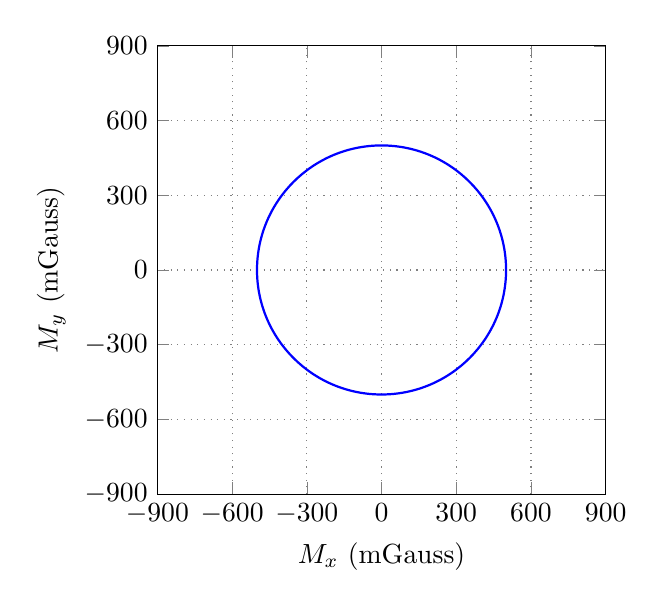
\begin{tikzpicture}
        \begin{axis}[
            axis equal image,
            grid=both,
            grid style={dotted, gray},
            xmin=-900, xmax=900,
            ymin=-900, ymax=900,
            xlabel={$M_x$ (mGauss)},
            ylabel={$M_y$ (mGauss)},
            xtick={-900,-600,-300,0,300,600,900},
            ytick={-900,-600,-300,0,300,600,900},
        ]

        % Plot the circle as an arc
        \draw[blue, thick] (axis cs: 0,0) circle [radius=500];
    \end{axis}
\end{tikzpicture}}
        \caption{Disturbance free}
        \label{fig:meas-mag-free}
    \end{subfigure}
    \begin{subfigure}{0.4\textwidth}
        \resizebox{0.7\textwidth}{!}{
        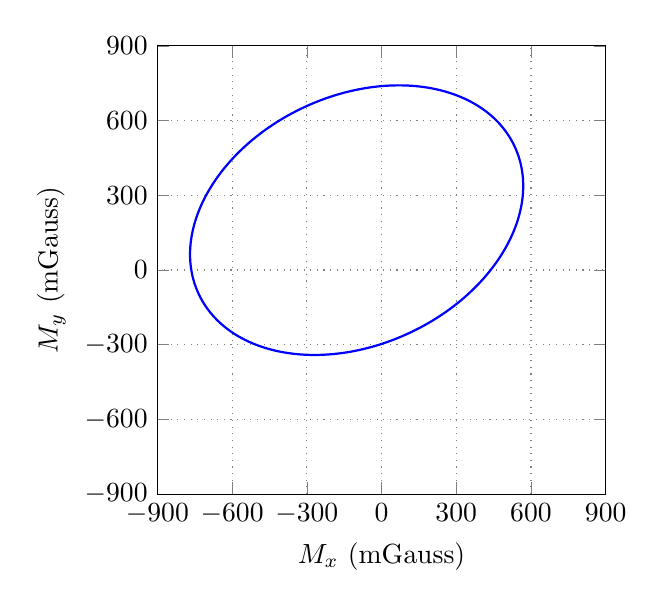
\begin{tikzpicture}
        \begin{axis}[
            axis equal image,
            grid=both,
            grid style={dotted, gray},
            xmin=-900, xmax=900,
            ymin=-900, ymax=900,
            xlabel={$M_x$ (mGauss)},
            ylabel={$M_y$ (mGauss)},
            xtick={-900,-600,-300,0,300,600,900},
            ytick={-900,-600,-300,0,300,600,900},
        ]

         % Plot the ellipse with correct offset and rotation
        \draw[blue, thick, rotate around={25:(axis cs:-100,200)}] (axis cs:-100,200) ellipse [x radius=700, y radius=500];
    \end{axis}
\end{tikzpicture}}
        \caption{Hard and soft iron disturbances}
        \label{fig:meas-mag-dist}
    \end{subfigure}
    \caption[2D Visualization of the measured magnetic field.]{2D Visualization of the measured magnetic field \cite{vectornav2024}.}
    \label{fig:meas-mag}
\end{figure}

The model of the measured magnetic field with hard and soft iron biases $b_{HI}$ and $B_{SI}$ is 
\begin{equation}
    M = S_M^T ( B_{SI} S M_E^G + b_{HI} ) \label{eq:meas-mag}
\end{equation}
where Earths magnetic field vector $M_E^G$ is rotated into the body-fixed and then the sensor frame with $S_M^T$.
Hard calibration (Section \ref{sec:hard-calibration}) must account for both biases and sensor frame rotation.
The inverse transformation needed for initialization is 
\begin{equation}
    M_E^G = S^T ( B_{SI}^{-1} (S_M M - b_{HI} ) \label{eq:meas-mag-init}
\end{equation}

\subsubsection{Pressure - Barometer}
The barometer measures the local air pressure with the sensor bias as
\begin{equation}
    P = p + b_P
\end{equation}
Air temperature $T$ cannot be measured reliably from barometric sensor, and will therefore not be used.
The atmosphere is modelled in Section \ref{sec:model-atmosphere}.

\subsubsection{Canard angle - shaft encoder}
There is a rotary potentiometer mounted on the canard shaft.
This encoder measures the canard angle directly, and the resulting sensor signal $\delta_e$ is 
\begin{align}
    \delta_e = \delta
\end{align}
Any biases and scaling is calibrated for by the encoder handler, and the resulting signal is just noisy. 

\subsubsection{Attitude and Heading reference system}
Commercial motion sensor units often feature not only an IMU, which provides raw sensor data of accelerometer, gyroscope, and magnetometer, but are also an self-contained \emph{Attitude and Heading Reference System} (AHRS).
These AHRS use their own sensor fusion algorithms to provide the 3D sensor attitude, often as Euler angles $\Theta$ or Quaternions $Q$.
The sensor model is complex as it contains the sensor models of the internal sensors, and the (often proprietary) filter computation.
However, the output can be approximated as the true attitude with additional white noise, so
\begin{align}
    Q &= q_Q * q & q &= q_Q^{-1} * Q
\end{align}
where the sensor attitude is rotated against the rocket frame by the constant $q_Q$.
Commercial AHRS are reliable attitude references, however their accuracy in these highly dynamic flight conditions (such as $\geq 10$g launch acceleration) remains to be tested.


\subsubsection{Satellite navigation}
Position in 3D as well as ground speed and heading could be determined by GPS.
However, the nominal trajectory goes well outside operational limits of commercially available GPS receivers (a < 4.5g, alt < 18km, v < 515m/s, by the time the rocket is below the acceleration limit it is above the speed limit)\footnote{The altitude and velocity limits are imposed by the US International Traffic in Arms Regulations.}.
While a GPS may be useful for recovery purposes, it cannot be used during most of the ascent, and therefore the filter will not include GPS.

\subsection{Atmosphere and air data}
\label{sec:model-atmosphere}
The static pressure $p$, temperature $T$, density $\rho$, and the local speed of sound $c$ of the surrounding air vary with altitude, as shown in Figure \ref{fig:atmosphere}.
This air data model is used to predict the barometer measurements and the aerodynamic effects accurately.
The air at altitude $l$ is modelled according to the US standard atmosphere \cite{usstandardatmosphere1976, stengel2004} as
\begin{align}
    \ell &= \frac{ R_0 l }{ R_0 - l } \label{eq:model-atmos-geopot} \\
    T &= T_B - k_B (\ell-\ell_B) \label{eq:model-atmos-temperature}
\end{align}
\begin{align}
    p &= p_B \exp \left( \frac{-g_0}{R T_B} (\ell-\ell_B) \right) &
    p &= p_B \left( 1 - \frac{k_B}{T_B} (\ell-\ell_B) \right) ^\frac{g_0}{R k_B} \label{eq:model-atmos-pressure}
\end{align}
\begin{align}
    \rho &= \frac{p}{R T} \label{eq:model-atmos-density} \\
    c &= \sqrt{\gamma R T} \label{eq:model-atmos-mach}
\end{align}
where the index $B$ indicates a base value from Table \ref{tab:atmosphere}. 
The altitude above sea level (geometric altitude) $l$ is converted to the geopotential altitude $\ell$ for the atmospheric calculations, using the mean Earth radius $R_0 = 6356.77 \mathrm{km}$. The gravitational acceleration is $g = 9.81 \frac{\mathrm{m}}{\mathrm{s}^2}$.
The adiabatic index of air is $\gamma = 1.4$, and the specific gas constant of air is $R = 287.0579 \frac{\mathrm{J}}{\mathrm{kg K}}$.
To calculate the static air pressure, Equation \ref{eq:model-atmos-pressure} is split in two, where the left equation is only used for a zero lapse rate $k_B = 0$.
\begin{table}[ht]
\begin{center}
\begin{tabular}{c c c c c}
Layer & Altitude $\ell_B$ [m] & Pressure $p_B$ [Pa] & Temperature $T_B$ [K] & Lapse rate $k_B \text{ } [\frac{\mathrm{K}}{\mathrm{m}}]$  \\
\hline % \midrule
Troposphere & 0 & 101325 & 288.15 & 0.0065 \\
Tropopause & 11000 & 22632.1 & 216.65 & 0 \\
Stratosphere & 20000 & 5474.9 & 216.65 & -0.001 \\ 
Stratopause & 32000 & 868.02 & 228.65 & -0.0028 \\
\end{tabular}
\end{center}
\caption[Atmosphere base data]{US Standard Atmosphere base data, \cite{usstandardatmosphere1976}} \label{tab:atmosphere}
\end{table}

\begin{figure}[ht]
    \centering
    \begin{subfigure}{0.32\textwidth}
        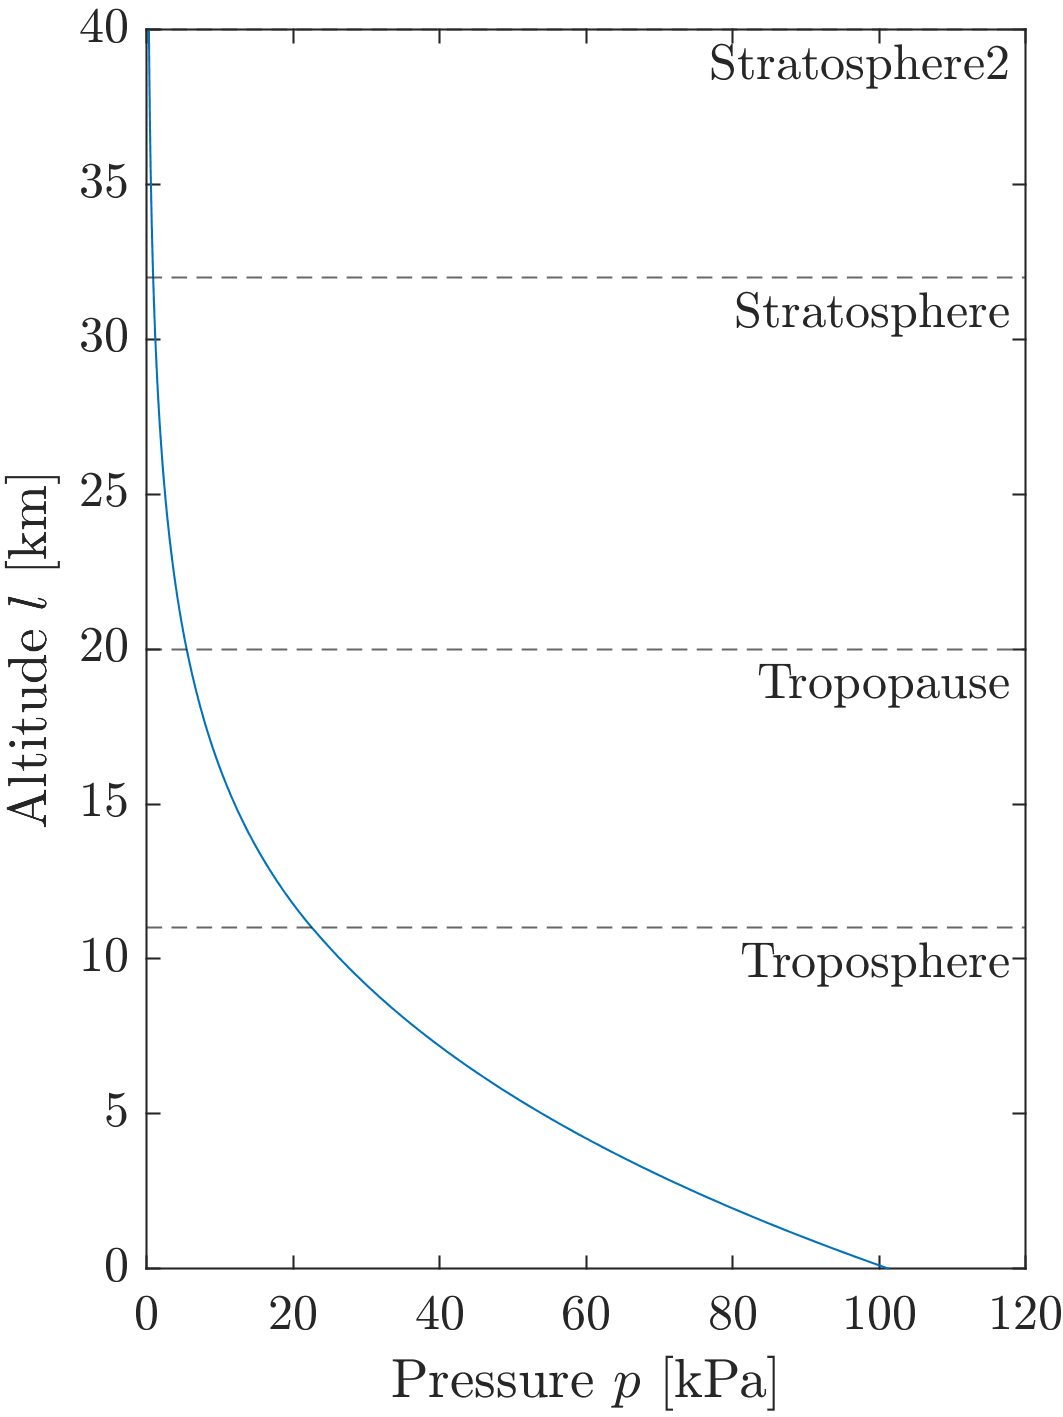
\includegraphics[width=0.9\textwidth]{images-design/model_atmosphere-pressure.png}
        \caption{Pressure}
        \label{fig:atmos-pressure}
    \end{subfigure}
    \begin{subfigure}{0.32\textwidth}
        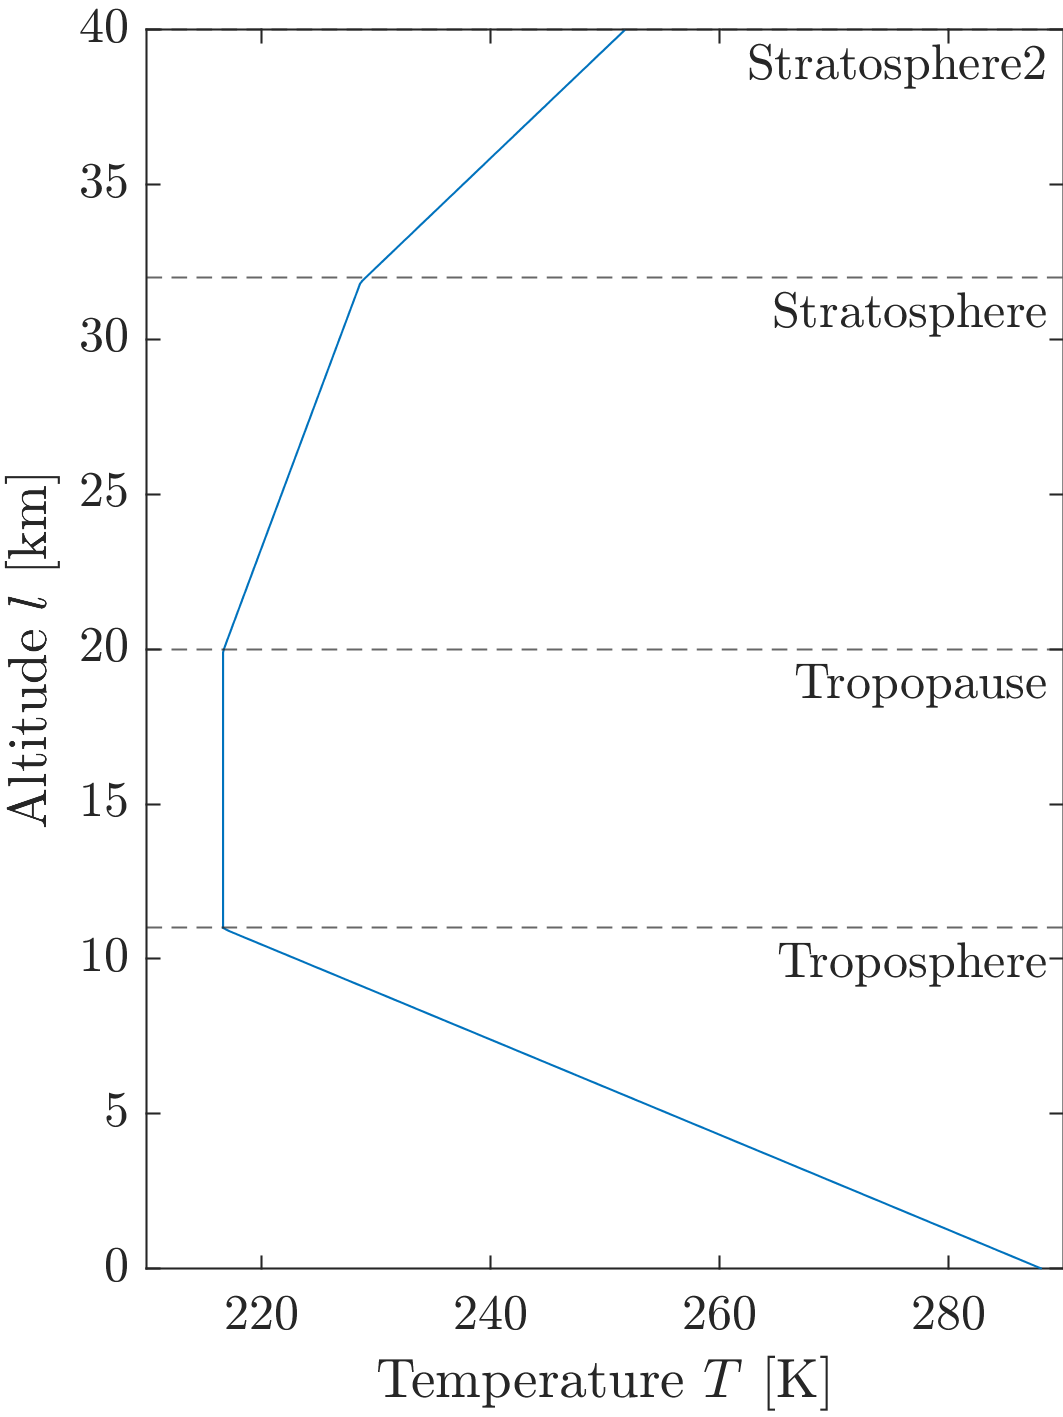
\includegraphics[width=0.9\textwidth]{images-design/model_atmosphere-temperature.png}
        \caption{Temperature}
        \label{fig:atmos-temperature}
    \end{subfigure}
    \begin{subfigure}{0.32\textwidth}
        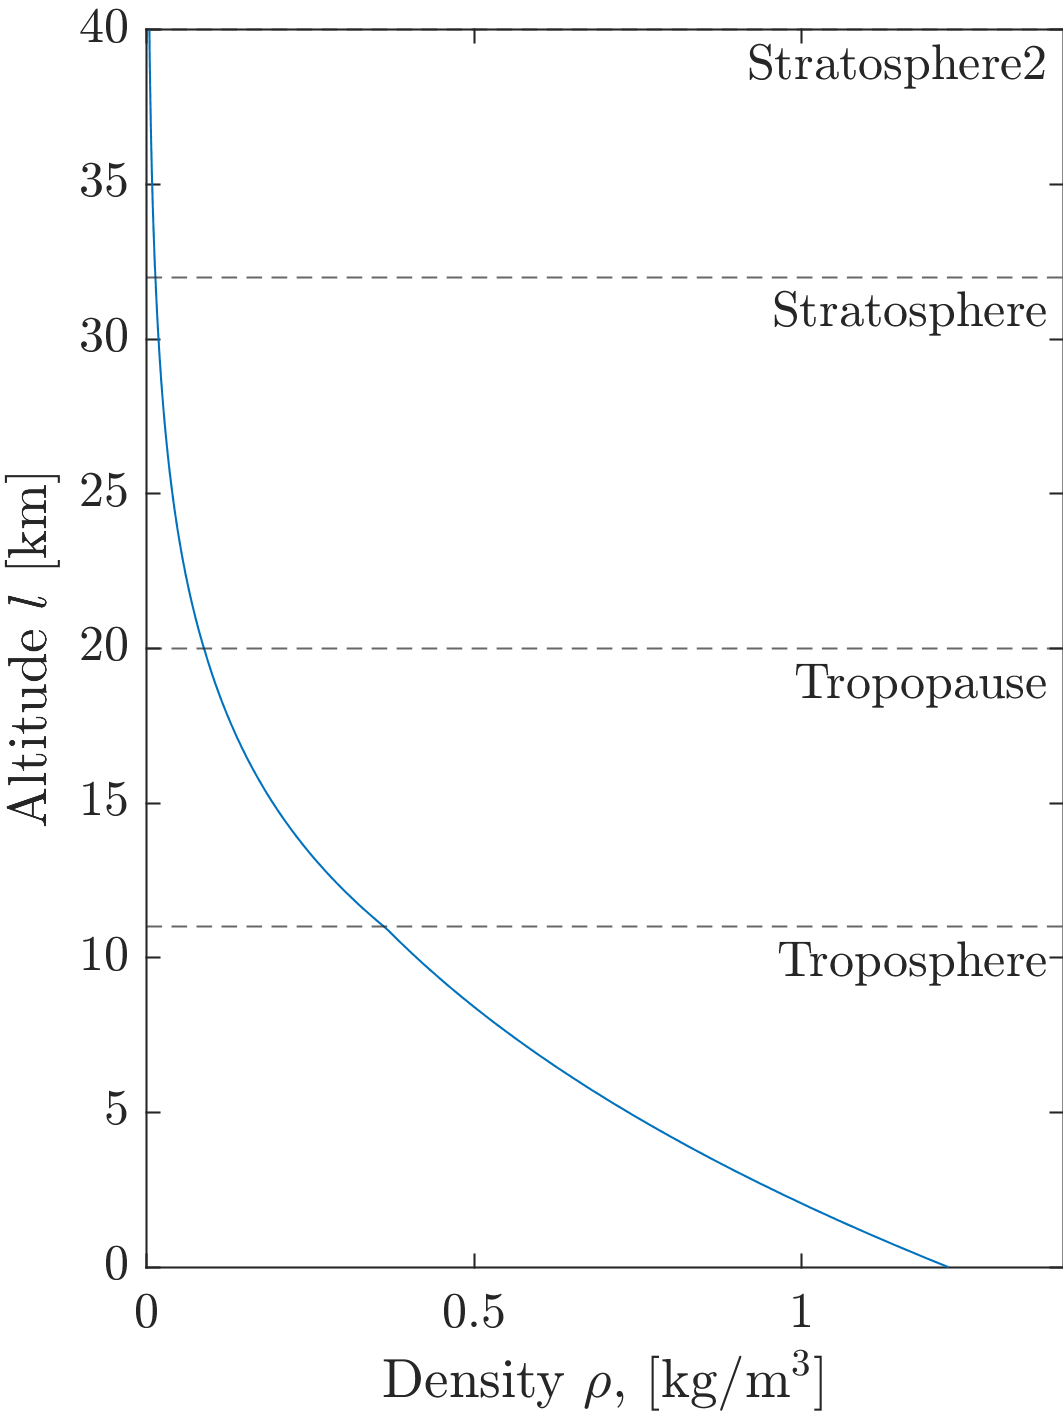
\includegraphics[width=0.9\textwidth]{images-design/model_atmosphere-density.png}
        \caption{Density}
        \label{fig:atmos-density}
    \end{subfigure}
    \caption[US standard atmosphere model]{Air value  variations with altitude, according to the US standard atmosphere model \cite{stengel2004}.}
    \label{fig:atmosphere}
\end{figure}

\subsubsection{Dynamic pressure \& Mach number}
The airspeed of the rocket is defined as $V_A = |v|$, which assumes no or only little wind disturbances\footnote{These are difficult to predict, and will thus act as disturbances on the rocket-estimator loop.}.
The dynamic pressure $\bar p$ and the Mach number $\mathrm{Ma}$ are defined as
\begin{align}
    \bar p &= \frac{1}{2} \rho V_A^2 
    &
    \mathrm{Ma} &= V_A / c
\end{align}
Where the dynamic pressure is the predominant factor in the aerodynamic forces and moments.
As the local speed of sounds varies with altitude, the Mach number for the same airspeed varies at different heights.
The Mach number has significant influence on the aerodynamic coefficients, and the location of the center of pressure.


\subsubsection{Angle of attack \& sideslip}
The incidence of the rocket relative to the oncoming airstream is defined with the \textit{angle of attack} $\alpha$ and the \textit{angle of sideslip} $\beta$.
As any wind gusts act as disturbances, both $\alpha$ and $\beta$ are defined from the velocity vector of the rocket in the body-fixed frame, as seen in Figure \ref{fig:model_alpha-beta}.
The angles are therefore
\begin{align}
        \alpha &= \mathrm{atan2}(v_z, \, v_x) &  \beta &= - \mathrm{atan2}(v_y, \,v_x)
\end{align}
Because the rocket is passively stable to movement in the forward direction (as determined by the Flight Dynamics subsystem), this can be approximated as
\begin{align}
    v_x &> 0 & v_x &\leq 0 \nonumber \\
    \alpha &\approx v_z/v_x  & \alpha &\approx \pi/2 \\
    \beta &\approx - v_y/v_x & \beta &\approx - \pi/2
\end{align}

\begin{figure}[ht]
    \centering
    \resizebox{0.25\textwidth}{!}{
    \begin{tikzpicture}[scale=0.65, every node/.style={scale=0.2}, auto, node distance=1.5cm,>=latex']
        \tikzstyle{every node}=[font=\LARGE]

		%origin
		\coordinate(o) at (0,0) {};

		%earth coordinates
 		\node (X) at (0,12) {$x^B$};
        \draw [ ->, dash dot] (o) -- (X);
        \node (Y) at (-6,-3) {$y^B$};
        \draw [ ->, dash dot] (o) -- (Y);
		\node (Z) at (8,-4) {$z^B$};
        \draw [ ->, dash dot] (o) -- (Z);
        		
		%box
		\coordinate(xx) at (0,10) {};
		\coordinate(yy) at (-4,-2) {};        
		\coordinate(zz) at (6,-3) {};
		\coordinate(yz) at (2,-5) {};
		\coordinate(xy) at (-4,8) {};
		\coordinate(xz) at (6,7) {};
		\coordinate(xyz) at (2,5) {};
		\draw [loosely dotted] (yy) -- (yz);
		\draw [loosely dotted] (zz) -- (yz);
		\draw [loosely dotted] (xx) -- (xy);
		\draw [loosely dotted] (yy) -- (xy);
		\draw [loosely dotted] (xx) -- (xz);
		\draw [loosely dotted] (zz) -- (xz);
		\draw [loosely dotted] (xy) -- (xyz);
		\draw [loosely dotted] (xz) -- (xyz);
		\draw [loosely dotted] (yz) -- (xyz);
        		
		%body coordinates		
		\node (x) at (2.2,5.5) {$v$};
		\draw [very thick, ->] (o) -- (x);
		\draw [dashed, ->] (o) -- (xy);
		\draw [dashed, ->] (o) -- (xz);
        \draw [very thick, ->] (o) -- (xx);
        \draw [very thick, ->] (o) -- (yy);
        \draw [very thick, ->] (o) -- (zz);

        \node (X) at (0.7,10.5) {$v_x$};
        \node (Y) at (-3.3,-0.9) {$v_y$};
		\node (Z) at (5.3,-1.9) {$v_z$};
      
        %angles
        \draw [very thick, ->] (0,8) arc (90:50:8);  
        \node (alpha) at (2.8,8.2) {$\alpha$}; 
        \draw [very thick, ->] (0,7) arc (90:116:7); 
        \node (beta) at (-1.5,7.5) {$\beta$}; 
\end{tikzpicture}}
    \caption[Diagram of the aerodynamic angles]{Diagram of the aerodynamic angles $\alpha$ and $\beta$ in the body-fixed coordinate frame}
    \label{fig:model_alpha-beta}
\end{figure}


\subsection{Aerodynamics}
The rocket dynamics have external forces and torques acting on the body, which are described here.
Note that the forces are described here, but the filter uses accelerometer data in the dynamics model, making the force computations unnecessary. 
The model could also be used not as a filter, but as a flight simulation, where explicit force equations would be used.
The external torques are still important however, as they couple the some unmeasured states to the angular velocity measurements.

\subsubsection{Forces and moments}
Most of the external forces and torques acting on the rocket will stem from aerodynamics.
The effect of rocket body geometry, including fins and nosecone, can be approximated using Barrowman's method \cite{barrowman1967}.

Any aerodynamic force for each component $^i$ is defined as 
\begin{align}
    \mathcal{F}^{\,i} &= \bar p \, C^i_{...} A^i 
\end{align}
where the aerodynamic coefficient (lift $C_L$, normal $C_N$, drag $C_D$, roll $C_l$) and reference area $A^i$ depend on the geometry of the component, and the lift coefficient encompasses information about the incidence angles. 

The torque produced by the aerodynamic forces is determined by the vector of the aerodynamic forces, acting through the the \textit{center of pressure} and producing a moment around the center of gravity as 
\begin{align}
    \mathcal{T}^{\, i} &= \mathcal{F}^{\, i} \times d^{\, i}
\end{align}
where $d^{\, i}$ is the vector from the center of pressure to the center of gravity (direction matters!).


The total aerodynamic forces and moments are 
\begin{align}
    \mathcal{F}_A &= \sum_i \mathcal{F}^{\,i} 
    & 
    \mathcal{T}_A &= \sum_i \mathcal{T}^{\,i}
\end{align}
For reference, later used coefficients are listed in Table \ref{tab:aero-coeff}.
\textit{Derivatives} are often used in aerospace control literature and encompass the force/torque and the corresponding inertia, partially differentiated around a variable $_i$.

\begin{table}[ht]
\begin{center}
\begin{tabular}{l l}
Symbol & Name \\
\hline
$C^\text{can}_{L_\delta}$ (in state notation $C_L$) & Lift coefficient, canards \\
$L_\delta$ & Roll control derivative \\
$C^\text{fins}_{l_{\omega_x}}$ &  Roll damping coefficient, fins \\
$L_{\omega_x}$ & Roll damping derivative, fins \\
$C_{N_\alpha}$ & Normal force coefficient, entire rocket
\end{tabular}
\end{center}
\caption{Aerodynamic parameters} \label{tab:aero-coeff}
\end{table}

\subsubsection{Canard airfoil theory}
\textit{A more in-depth development has been done by Luca Scavone, lead of the flight dynamics subsystem \cite{team-flight-luca}}.
The coefficient of lift is approximated using thin airfoil theory \cite{stengel2004}.
The canards have a triangular (\textit{delta} $\Delta$) shape, with a high \textit{sweep angle} $\Lambda$. 
The lift coefficient depends on the Mach number of the rocket, as the flow behaviour starts to change near sonic speed.
Protruding geometries of the rocket body, such as the canards, have shock waves attached to them if the surrounding flow is supersonic.
At higher speeds, these shock waves angle more and more backwards. 
The characteristic Mach angle is defined as $\mu = 0$ for $\mathrm{Ma} < 1$ and for $\mathrm{Ma} \geq 1$ as \cite{stengel2004}
\begin{equation}
    \mu = \arccos(\frac{1}{\mathrm{Ma}})
\end{equation}
For a subsonic leading edge $\mu \leq \Lambda$ (i.e. the canard is more acute than the Mach cone), the coefficient of lift is empirically determined \cite{stengel2004} as Equation \ref{eq:model_airfoil-subsonic}.
When the Mach cone is steeper than the canard leading edge $\mu > \Lambda$, the coefficient of lift follows a simpler law \cite{stengel2004} in Equation \ref{eq:model_airfoil-super}.
\begin{align}
    \mathrm{Ma} &<  1: & C_{L_\delta} &= 2 \pi\cot(\Lambda)
    \\
    \mu &\leq \Lambda : & C_{L_\delta} &= \frac{2 \pi^2 \cot(\Lambda)}{\pi + \eta (0.38 + 2.26 \eta - 0.86 \eta^2)} \quad \text{with} \quad \eta = \frac{\cot(\Lambda)}{\cot(\mu)} \label{eq:model_airfoil-subsonic} 
    \\
    \mu &> \Lambda : &C_{L_\delta} &= \frac{4}{\sqrt{\mathrm{Ma}^2-1}} \label{eq:model_airfoil-super}
\end{align}
For small deflection $\delta < 10^\circ$ of the canard surfaces, the coefficient of lift is proportional to the deflection angle, so $C_L = C_{L_\delta} \delta$.
The equations for the coefficient of lift are shown in the Figures \ref{fig:airfoil}.
Figure \ref{fig:airfoil-angles} shows the coefficient $C_{L_\delta}$ and Mach angle $\mu$ for an exemplary sweep angle of 60°, 

\begin{figure}[ht]
    \centering
    \begin{subfigure}{0.49\textwidth}
        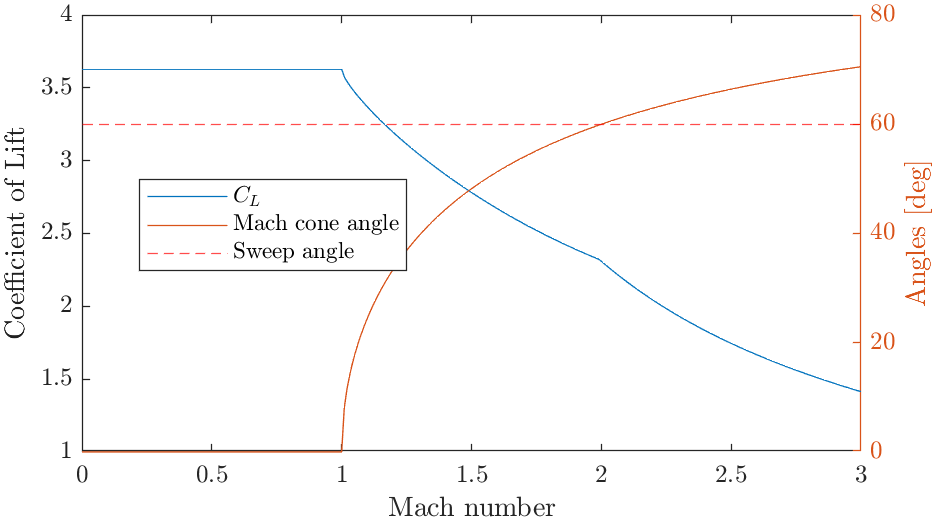
\includegraphics[width=0.9\textwidth]{images-design/airfoil_angles.png}
        \caption{Lift coefficient and Mach cone angle vs. Mach number, for 60° sweep angle}
        \label{fig:airfoil-angles}
    \end{subfigure}
    \begin{subfigure}{0.49\textwidth}
        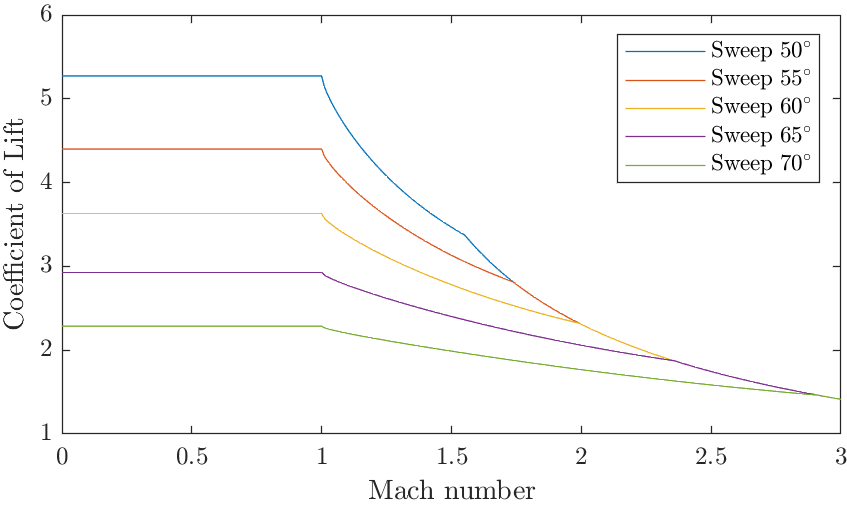
\includegraphics[width=0.9\textwidth]{images-design/airfoil_sweeps.png}
        \caption{Lift coefficients vs. Mach number, for different sweep angles}
        \label{fig:airfoil-sweeps}
    \end{subfigure}
    \caption[Swept delta airfoil theory]{Coefficient of lift for swept delta airfoils}
    \label{fig:airfoil}
\end{figure}


\subsubsection{Roll forces and roll moments}
The resulting force of one canard is $\mathcal{F}^\text{can}_1 = \bar p \, C^\text{can}_{L_\delta} \delta A^\text{can}_1$, which is orthogonal to the $x^B$ vector, and acts on the center of pressure of the canard surface.

\begin{figure}[ht]
    \centering
    \resizebox{0.6\textwidth}{!}{
    \begin{tikzpicture}[scale=1.3, every node/.style={scale=0.3}, auto, node distance=1.5cm,>=latex']
\tikzstyle{every node}=[font=\normalsize]

% Draw axes
\draw[thick,->, dash dot] (0,0) -- (4,0) node[anchor=north] {$x^B$};
\filldraw (0,0) circle (0.1em);
\draw (0,0) circle (0.2em);
\node (Y) at (-0.3,0.3) {$y^B$};
\draw[thick,->, dash dot] (0,0) -- (0,-2) node[anchor=east] {$z^B$};

% Draw canard
\draw[very thick] (1,-0.5) -- (3,0.5) node[pos=1, above right] {Canard};
\filldraw (2,0) circle (0.1em);

% Draw airflow arrow
\draw[thick,->] (8,0) -- (4.5,0.2) node[pos=0, below] {Airflow};
\draw[thick,->] (8,0.5) -- (4.5,0.7);
\draw[thick,->] (8,-0.5) -- (4.5,-0.3);
\draw[thick,->] (8,-1) -- (4.5,-0.8);


% Draw force vector
\draw[thick,->] (2,0.1) -- (2,2) node[midway, left] {$+\mathcal{F}^\text{can}_1$};

% Draw delta angle
\draw[->] (2.7,0) arc[start angle=0,end angle=26.57,radius=0.7];
\node at (3,0.2) {$+\delta$};

% Draw rocket body
\draw[thin] (6,-1.5) -- (-1,-1.5) node[pos=0.2, below] {Rocket body};
\draw[thin] (6,1.5) -- (-1,1.5);

\end{tikzpicture}}
    \caption[Diagram of the canard angle]{Diagram of the canard angle $\delta$ in the body-fixed coordinate frame. Modelled after \cite{siouris2004}.}
    \label{fig:model_delta}
\end{figure}

As the canards are of equal size, and move in equal and opposite angles, the normal force on the rocket body cancels out (for small angles of attack of the rocket body), it remains a net moment about the rocket $x$-axis.
The forces and moments produced by the canards are thus 
\begin{align}
    \mathcal{F}^\text{can} &= \begin{bmatrix} 0 \\ 0 \\ 0 \end{bmatrix}
    & 
    \mathcal{T}^\text{can} &= \begin{bmatrix} \bar p \, C^\text{can}_{L_\delta} \delta A^\text{can} d^\text{can}_y 
    \\ 0 \\ 0 \end{bmatrix} \label{eq:model-aero-canards}
\end{align}
where $A^\text{can}$ is the total planform area of all canards and $d^\text{can}_y$ is the distance between the rocket roll axis $x^B$ and the center of pressure of one of the canards (i.e. the moment arm).
The instantaneous roll acceleration of the canards can be written with the roll control derivative $L_\delta$ as 
\begin{align}
    \dot \omega_x &= \mathcal{T}^\text{can}_x / J_x = L_\delta \, \delta
    & 
    L_\delta &= \bar p \, C^\text{can}_{L_\delta} A^\text{can} d^\text{can}_y / J_x
\end{align}
which simplifies notation of the roll dynamics as shown in Section \ref{sec:model_controller}.

The roll forces of the rocket body are dominated by fin effects, namely roll forcing from misalignment, and roll damping from the fin wake of a rolling rocket. 
The roll forcing is difficult to predict if the fin misalignment is not exactly know, so any forcing will be treated as disturbances acting on the rocket.
The roll forcing is therefore neglected, but the roll damping is 
\begin{align}
    \mathcal{F}^\text{fins} &= \begin{bmatrix} 0 \\ 0 \\ 0 \end{bmatrix}
    & 
    \mathcal{T}^\text{fins} &= \begin{bmatrix} \bar p \, C^\text{fin}_{l_{\omega_x}} \omega_x A^\text{fins} d^\text{fins}_y \\ 0 \\ 0 \end{bmatrix}
\end{align}
The instantaneous roll acceleration from roll damping of the fins can be written with the roll damping derivative $L_{\omega_x}$ as 
\begin{align}
    \dot \omega_x &= \mathcal{T}^\text{fins}_x / J_x = L_{\omega_x} \, \omega_x
    & 
    L_{\omega_x} &= \bar p \, C^\text{fins}_{L_{\omega_x}} A^\text{fins} d^\text{fins}_y / J_x
    \label{eq:model-aero-fins}
\end{align}


\subsubsection{Normal forces and moments}
Barrowman's method can be employed to derive the location of the center of pressure and the normal force coefficient, for each component of the rocket body \cite{barrowman1967, niskanen2009}.
Accurate parameters are determined by the Flight Dynamics subsystem.

Important effects are aerodynamic drag, the total normal force and moment, the roll control and roll damping coefficients, and their respective centers of pressure.

The normal forces and the resulting pitch/yaw torques are 
\begin{align}
    \mathcal{F}^\text{normal} &= 
    \begin{bmatrix} 
    0 \\ 
    \bar p \, C_{N_\alpha} \beta A^\text{ref} \\ 
    \bar p \, C_{N_\beta} \alpha A^\text{ref}
    \end{bmatrix}
    & 
    \mathcal{T}^\text{normal} &= 
    \begin{bmatrix} 
    0 \\
    \bar p \, C_{N_\alpha} \alpha A^\text{ref} d^\text{ref} \\
    \bar p \, C_{N_\beta} \beta A^\text{ref} d^\text{ref}
    \end{bmatrix} \label{eq:model-aero-normal}
\end{align}


% \subsubsection{Propulsion}
% The forces and moments produced by the engine are determined by the Propulsion subsystem.
% As we cannot predict thrust misalignment, it is assumed zero with any misalignment acting as disturbances, so the moment produces by the engine is zero.
% Any sloshing or pogo-effect is too complex to model here, and will be neglected.
% This leaves an ``unknown'' axial propulsion force as some function of the engine performance $F_\text{engine}$, so
% \begin{align}
%     \mathcal{F}_P = \begin{bmatrix}
%         \mathcal{F}_\text{engine}(t, \rho, ...) \\ 0 \\ 0
%     \end{bmatrix}
% \end{align}

% \subsubsection{Rail constraints}
% The rocket is attached to the launch rail for the first few meters of altitude, constraining the rocket to one degree of freedom (translating upwards).
% This effect only acts during the first few fractions of a second, and will therefore be neglected for the flight model.
% However, as long as the rocket is (knowingly) on the launch rail, the movement constraints can be used to initialize the state, and to determine sensor biases. 

\subsection{Actuators}
\textit{The mechanical design of the canard actuating system has been done by Ben Pickens, Co-lead of the controls subsystem \cite{team-controls-ben}}.
The actuation system, shown in Figure \ref{fig:model-actuator-cad}, rotates two canards in opposite directions by equal amounts, thus providing a roll-only torque on the rocket.
The actuation is provided by a servo motor, driving the canard shafts via bevel gears.
It acts as a position control element, which provides a calculated torque to reach the commanded shaft angle. 
To provide accurate position feedback to the controller / state estimation, rotary potentiometers are mounted on the canard shafts.
\begin{figure}[ht]
    \centering
    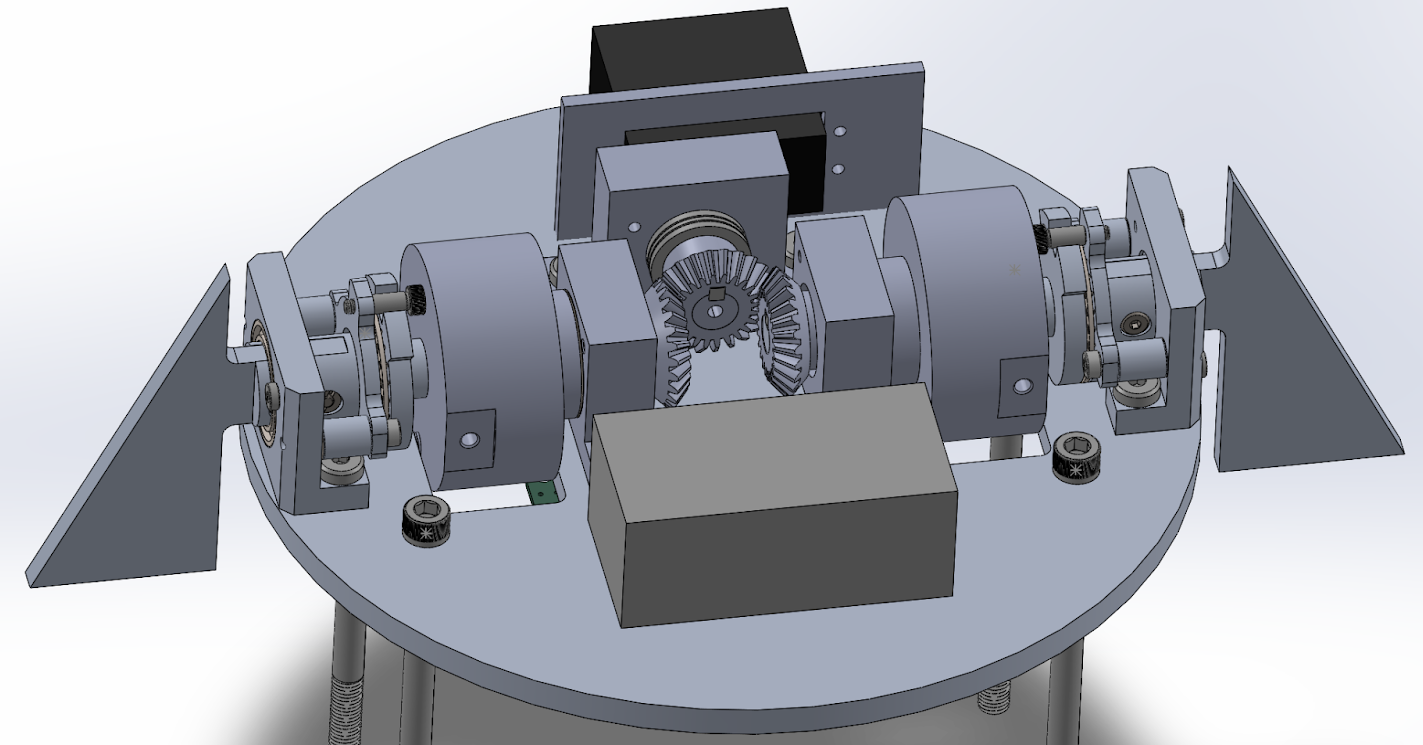
\includegraphics[width=0.6\linewidth]{images-design/actuator_cad.png}
    \caption[Mechanical design of the actuator]{Mechanical design of the canards actuation assembly \cite{team-controls-ben}.}
    \label{fig:model-actuator-cad}
\end{figure}

\subsubsection{Actuator dynamics}
%The drive train is made up of a servo motor, the servo and canard shafts, and the gearing between them.
The internal control loop of the servo has some higher order dynamics, non-linearity in a maximum angle and limited speeds, and some dead-time before it starts responding.
A reasonable approximation to use for the controller and state estimation models would be a first or second order linear system, the former is chosen to keep the state vector small (and thus the filter computations shorter).

The first order system with the actual canard angle $\delta$, the commanded servo angle $\delta_u$, and the gear ratio between the servo and the canard $\beta_\delta$, has the form
\begin{equation}
    \dot \delta = -\alpha_\delta (\delta - \beta_\delta\delta_u)
\end{equation}
The dynamics are dominated by the time constant $\alpha_\delta$, which describes how fast the canard angle responds to a servo command. 
Solving the ODE results in the step response
\begin{align}
    \delta(t) = (1-\mathrm{e}^{-\alpha_\delta t}) \beta_\delta \delta_u
\end{align}
Notably, when no non-linearity is present, i.e. as long as the servo speed limit is not reached, the response time does not depend on the commanded angle $\delta_u$.

The first order response is fitted to the measured actuator response by adjusting the time constant.
The gear ration is assumed to be $\beta_\delta = 1$ from now on, later equations need to be adjusted if that should change. 

\textit{Todo. Insert plots here.}


\subsection{Estimator model equations}
\label{sec:model_estimator}
The rocket model is made up of algebraic and differential equations \cite{zipfel2007, lewis2008, stevens2015}, represented in \textit{state-space} as \cite{lewis2008, stevens2015} (Equations \ref{eq:model-equation-f} and \ref{eq:model-equation-h})
\begin{align}
    \dot x &= f(t, x, u) \nonumber \\  y &= h(t, x, u) \nonumber
\end{align}  
with the state $x$, measurement output $y$, and control input $u$.
Here the state equation $f$ and the output equation $h$ are nonlinear functions.


\subsubsection{States $x$}
From textbooks \cite{zipfel2007, stevens2015, tewari2011},  lectures \cite{theis2023}, papers \cite{minh2012, theis2015}, the industry standard for choosing states of aeronautical vehicles is using attitude angles, attitude rates, velocity, and position. 

Here, position is reduced to altitude only, as longitude and latitude are not required and cannot be measured without GPS\footnote{Commercial GPS lockouts are expected at our speed and altitude, to prevent guided missile design.}. 
The entire state vector is then
\begin{equation}
    x =  \begin{bmatrix}
    q & \omega & v & l & C_L & \delta
    \end{bmatrix}^T
    \label{eq:model-state-vector}
\end{equation}
with the attitude represented as quaternions $q = \begin{bmatrix} q_w & q_x & q_y & q_z \end{bmatrix}^T$, the angular velocity in the body-fixed frame $\omega = \begin{bmatrix} \omega_x & \omega_y & \omega_z \end{bmatrix}^T$ (body rates)\footnote{In literature the body rates are often depicted as $\omega_x = p$, $\omega_y = q$, and $\omega_z = r$. As this may be confusing, we'll stick with $\omega_i$ for the rates in this documentation.}, the velocity in the body-fixed frame $v = \begin{bmatrix} v_x & v_y & v_z \end{bmatrix}^T$, and the altitude over sea level $l$. 
Additionally, the canards have the coefficient of lift $C_L$ as we are unsure about the aerodynamic behaviour of the canards (and as a state, the coefficient can be estimated), and the angle-of-attack $\delta$ which is used to carry first order actuator dynamics.

\subsubsection{Measurements $y$}
The measurements arrive in the measurement vectors
\begin{align}
    y_{IMU} &=  \begin{bmatrix}
    \Omega & M & P
    \end{bmatrix}^T 
    \\
    y_{encoder} &=  \begin{bmatrix}
    \delta_e
    \end{bmatrix}
    \\
    y_{AHRS} &=  \begin{bmatrix}
    Q
    \end{bmatrix}
\end{align}
with measured body rates from the rate gyroscope $\Omega = \begin{bmatrix} \Omega_x & \Omega_y & \Omega_z \end{bmatrix}^T$, the magnetic field measurement $M = \begin{bmatrix} M_x & M_y & M_z \end{bmatrix}^T$ (which can be transformed to attitude\footnote{The inverse transformation is not unique as it is invariant about the field direction, but we can’t use the accelerometer in free flight to find the gravity vector.}) from the magnetometer, additionally the static air pressure $P$ is provided by the barometer (the temperature $T$ is not used, as its measurement is unreliable).
The accelerometer data $A$ will be provided to the filter in the input vector, as this simplifies calculations.\footnote{This is quite common practice}
The encoder signal $\delta_e$ also arrives in its measurement vector, and so does a possible attitude reference from an AHRS.
Each one of these measurement vectors has its own measurement model.

\subsubsection{Inputs $u$}
The control input vector is the commanded canard angle to the actuator $\delta_u$ and, as stated in the previous paragraph, the  accelerometer data $A = \begin{bmatrix} A_x & A_y & A_z \end{bmatrix}^T$.

As the acceleration is not a state, %and cannot be directly computed from the other states (aerodynamic modelling is too indirect), 
it is used in the state prediction step instead of the correction step. 
The measured acceleration $A$ enters the prediction function as a control input.
As these measurements do not enter the filter in the classical way, their weighting of the expected covariances has to happen in the prediction model.
The transformation to the body-fixed body-centered frame from Equation \ref{eq:meas-accel} is performed first, after which the $a_i$ will be weighted and then fed to Equation \ref{eq:meas-veldot}.
\begin{equation}
    u =  \begin{bmatrix}
    \delta_u & A
    \end{bmatrix}^T
    \label{eq:model-input-vector}
\end{equation}
The actual canard angle is represented as the state $\delta$, to account for actuator dynamics.
The computation from desired canard angle to servo command should be performed in the controller. 

\subsubsection{Dynamics model}
\begin{equation}
    \dot{\hat x} = f(t, \hat x, u) \nonumber
\end{equation}
predicts the time derivative of the state vector, $\dot{\hat x}$ (Equation \ref{eq:model-state-vector}), using the control input $u$ (Equation \ref{eq:model-input-vector}), and the following model equations:
\begin{itemize}
    \item Attitude: \ref{eq:quaternion-deriv}
    \item Rates: \ref{eq:model-rate-deriv}
    \item Velocities: \ref{eq:meas-veldot} for filtering and \ref{eq:model-vel-deriv} for simulation
    \item Position/Altitude: \ref{eq:model-pos-deriv}
    \item Canard coefficient: 1st order dynamics $\dot C_L = -\alpha_c (C_L - C_{L\text{, theory}})$, airfoil theory Equations \ref{eq:model_airfoil-subsonic} and \ref{eq:model_airfoil-super}
    \item Canard angle: 1st order dynamics $\dot \delta = -\alpha_\delta (\delta - \delta_u)$
\end{itemize}

\subsubsection{Measurement model} 
\begin{equation}
    \hat y = h(t, \hat x, u) \nonumber
\end{equation}
predicts the sensor outputs $\hat y$ from the current state estimate $\hat x$, and the model equations:
\begin{itemize}
    \item Gyroscope: \ref{eq:meas-gyro}
    \item Accelerometer: used in state prediction as \ref{eq:meas-accel} and \ref{eq:meas-veldot}
    \item Magnetometer: \ref{eq:meas-mag}
    \item Barometer: \ref{eq:model-atmos-temperature} to \ref{eq:model-atmos-mach}
\end{itemize}

\subsection{Controller model equations}
\label{sec:model_controller}
The model used for controller synthesis must be linear, time-invariant, and controllable.
Linear time-invariant state-space models can be derived by linearizing the equations $f$ and $h$ around some design point $(t_0, x_0, u_0)$, which results in the equations (Equations \ref{eq:model-linear-state} and \ref{eq:model-linear-meas})
\begin{align}
    \dot x = A (x-x_0) + B (u-u_0) \nonumber \\
    y = C (x-x_0) + D (u-u_0) \nonumber
\end{align}
These equations may be employed around a collection of design points $\{ t_s, x_s, u_s \}$ do account for varying parameters of the matrices ($A,B,C,D$).

As the model must be controllable, it makes some simplifications compared to Section \ref{sec:estimator}.
This is because the actuating canards can only produce a roll torque, i.e. a moment about the $x$-axis, but cannot directly influence other states, e.g. pitch and yaw rates or altitude.
This results in the full model from Section \ref{sec:model_estimator} not being controllable, i.e. we cannot use the pole placement method to arbitrarily choose our desired dynamics.
Additionally, the full uncontrollable model includes uncontrollable modes, which make analysis of the control loop more cumbersome. 
To solve this problem, the ``full'' state dynamics are projected unto the controllable subspace -- i.e. the number of states are reduced to those that can be influenced, and the model is simplified.  


\subsubsection{Simplifications}
The cross coupling term $\omega \times J \omega$ is neglected, as the rocket is assumed to have an approximately diagonal $J$, and the roll dynamics are much faster than the pitch/yaw dynamics. 
The attitude kinematics of the quaternion are neglected to assume that the rate of the roll angle is the roll rate, so $\dot \phi = \omega_x$.
This roll angle $\phi$ is computed from the quaternions in the Estimator; $\phi = \mathrm{atan2}( S_{23}, S_{33} )$ as shown in Equation \ref{eq:quaternion2euler} (expressed here as entries of the rotation matrix).

The altitude and the velocity vector are not directly controllable, so they are removed from the controller model as well. 
To preserve the aerodynamics information, the velocity and altitude are combined to the dynamic pressure $\bar p$ acting on the rocket. 
The dynamic pressure and the canard coefficient $C_L$ are not states, but variable parameters of the model matrix $A$.
They are combined to the \emph{flight condition}
\begin{equation}
    x_{FC} = \begin{bmatrix} \bar p & C_L \end{bmatrix} \label{eq:controller-model-fc}
\end{equation}

\subsubsection{State-space representation}
The simplifications leave three state variables for the controller roll model, being roll angle, roll rate, and the canard deflection angle.
Thus the state vector $x_R$ of the roll model is 
\begin{align}
    x_R = \begin{bmatrix} \phi & \omega_x & \delta \end{bmatrix}^T
    \label{eq:controller-model-state}
\end{align}
As input to the system serves the commanded canard angle $\delta_u$, and all states are available as outputs due to the state estimation.
The resulting state-space model is then 
\begin{align}
    \dot x_R &= A(x_{FC}) \: x_R + B \delta_u 
    &
    y_R &= C x_R
    \label{eq:controller-model-ss}
\end{align}
with the matrices
\begin{align}    
    A &= \begin{bmatrix}
        0 & 1 & 0 \\
        0 & L_{\omega_x} & L_\delta \\
        0 & 0 & -\alpha
    \end{bmatrix}
    &
    B &= \begin{bmatrix}
        0 \\ 0 \\ \alpha
    \end{bmatrix}
    &
    C &= \begin{bmatrix} I_3 \end{bmatrix}
    \label{eq:controller-model-matrices}
\end{align}
where the roll control derivative is $L_\delta (\bar p,  \,  C_L)$, a function of dynamic pressure and the canard coefficient of lift, i.e. the flight condition.
Roll damping is modelled by the roll damping derivative $L_{\omega_x} (\bar p, \, C_{L \omega_x})$.
Roll damping originates almost entirely from fixed fins which resist turning - for freely rolling fins (a spin can), the damping derivative should be very small as approximately only the canards themselves damp rolling motion.
The 1st order actuator dynamics are accounted for with the $\delta$ state, and are characterized by the time constant $\alpha$, whose value should be determined by experimental system identification.
Any gear ratio between servo motor and canards may be expressed as a factor of the bottom entry of $B$ (here set to 1).